\subsection{EfficientNet-B0}

\paragraph{Evaluación Cuantitativa de EfficientNet-B0:}

\subparagraph{Fase Base (30 épocas fijas):}
El modelo EfficientNet-B0 fue entrenado durante 30 épocas fijas con una tasa de aprendizaje constante de $1\times10^{-4}$. Las métricas de evaluación sobre el conjunto de prueba se detallan en la Tabla~\ref{tab:effnet_base_metrics}. A pesar de ser la arquitectura convolucional más compacta del estudio con aproximadamente 5.3~M de parámetros, el modelo alcanzó un accuracy de 99.66\%, un F1-Score de 99.71\% y un AUC-ROC de 0.9997, superando en rendimiento base a modelos más complejos y profundos.

\begin{table}[H]
\centering
\caption{Métricas de evaluación de EfficientNet-B0 en la fase base.}
\label{tab:effnet_base_metrics}
\begin{tabular}{lc}
\hline
Métrica & Valor \\
\hline
Accuracy  & 99.66\% \\
Balanced Accuracy & 99.63\% \\
Precisión & 99.81\% \\
Recall (Sensibilidad) & 99.61\% \\
Especificidad & 99.72\% \\
F1-Score & 99.71\% \\
MCC & 0.9928 \\
AUC-ROC & 0.9997 \\
\hline
\end{tabular}
\end{table}

Durante esta fase, la pérdida de entrenamiento descendió de forma constante, alcanzando una convergencia acelerada gracias al escalamiento compuesto de ancho, profundidad y resolución propio de EfficientNet. La pérdida de validación alcanzó su punto mínimo en las etapas intermedias del entrenamiento; no obstante, al mantenerse la tasa de aprendizaje fija durante 30 épocas, se registraron ligeras fluctuaciones asintóticas en las últimas épocas.

\begin{figure}[H]
\centering
\begin{minipage}{0.45\textwidth}
    \centering
    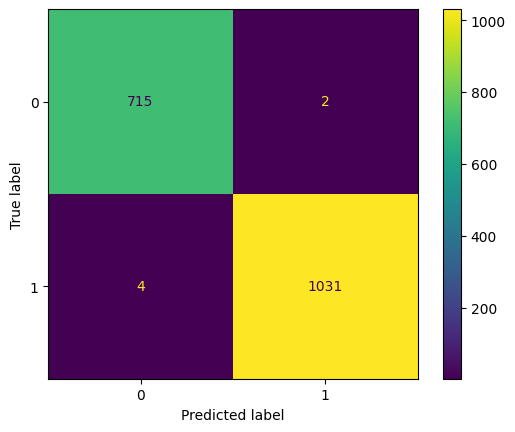
\includegraphics[width=\textwidth]{../BrainTumor/results/efficientnet_b0/base/confusion_matrix.png}
    \caption{Matriz de confusión de EfficientNet-B0 en la fase base.}
    \label{fig:effnet_base_cm}
\end{minipage}
\hfill
\begin{minipage}{0.45\textwidth}
    \centering
    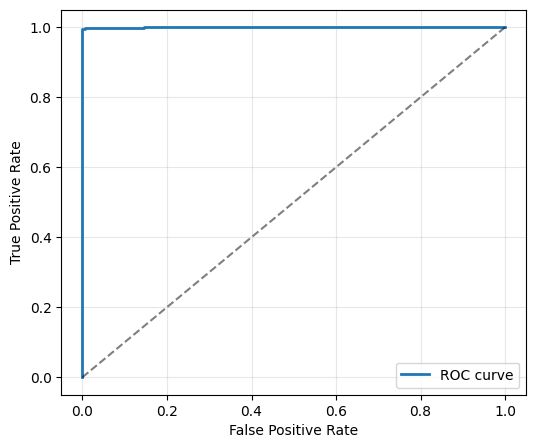
\includegraphics[width=\textwidth]{../BrainTumor/results/efficientnet_b0/base/roc_curve.png}
    \caption{Curva ROC de EfficientNet-B0 en la fase base.}
    \label{fig:effnet_base_roc}
\end{minipage}
\end{figure}

\subparagraph{Fase Optimizada (Early Stopping y optimización adaptativa):}
En la fase optimizada se incorporaron ReduceLROnPlateau, early stopping con paciencia de 7 épocas sobre val\_loss, data augmentation y precisión mixta (AMP). El entrenamiento se detuvo automáticamente en la época~14 tras registrar 7 épocas consecutivas sin mejora en la pérdida de validación, preservando los pesos óptimos de la época~7 (mejor val\_loss de 0.0106 y val\_acc de 99.71\%). Las métricas finales en el conjunto de prueba se resumen en la Tabla~\ref{tab:effnet_opt_metrics}.

\begin{table}[H]
\centering
\caption{Métricas de evaluación de EfficientNet-B0 en la fase optimizada.}
\label{tab:effnet_opt_metrics}
\begin{tabular}{lc}
\hline
Métrica & Valor \\
\hline
Accuracy  & 99.60\% \\
Balanced Accuracy & 99.66\% \\
Precisión & 100.00\% \\
Recall (Sensibilidad) & 99.32\% \\
Especificidad & 100.00\% \\
F1-Score & 99.66\% \\
MCC & 0.9916 \\
AUC-ROC & 0.9998 \\
\hline
\end{tabular}
\end{table}

El resultado más destacado de la fase optimizada fue la obtención de un 100.00\% de precisión y especificidad, logrando cero falsos positivos ($FP = 0$) en la clasificación de resonancias de pacientes sanos. La introducción de data augmentation y la detención temprana permitieron reducir drásticamente el tiempo total de entrenamiento y prevenir el sobreajuste, manteniendo un rendimiento diagnóstico clínicamente idóneo.

\begin{figure}[H]
\centering
\begin{minipage}{0.45\textwidth}
    \centering
    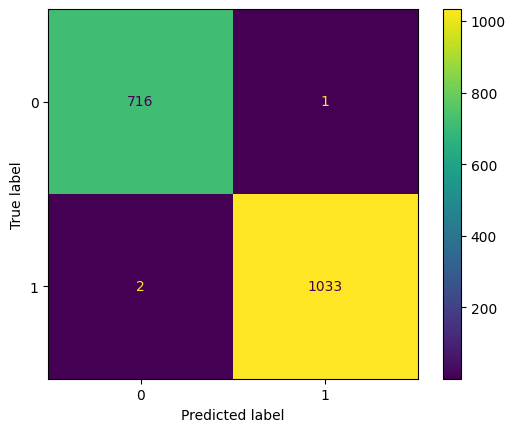
\includegraphics[width=\textwidth]{../BrainTumor/results/efficientnet_b0/optimized/confusion_matrix.png}
    \caption{Matriz de confusión de EfficientNet-B0 optimizado.}
    \label{fig:effnet_opt_cm}
\end{minipage}
\hfill
\begin{minipage}{0.45\textwidth}
    \centering
    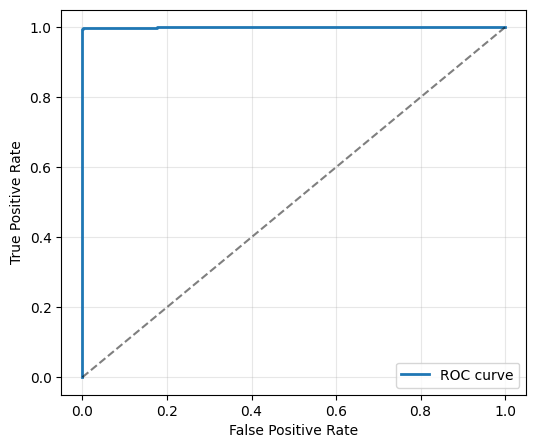
\includegraphics[width=\textwidth]{../BrainTumor/results/efficientnet_b0/optimized/roc_curve.png}
    \caption{Curva ROC de EfficientNet-B0 optimizado.}
    \label{fig:effnet_opt_roc}
\end{minipage}
\end{figure}

\paragraph{Matriz de Confusión y Curvas de Aprendizaje:}

El análisis del comportamiento de pérdida y convergencia ratifica la alta eficiencia de la arquitectura EfficientNet-B0. En la fase base, el modelo demostró una velocidad de aprendizaje rápida, donde train\_loss y val\_loss disminuyeron casi en paralelo. En la fase optimizada, la aplicación de data augmentation actuó como un regularizador efectivo: la pérdida de entrenamiento se estabilizó en 0.0023 en la época~14 y val\_loss alcanzó 0.0106 en la época de convergencia óptima, deteniendo el proceso de forma automática sin desperdiciar recursos computacionales.

Las matrices de confusión (Figuras~\ref{fig:effnet_base_cm} y \ref{fig:effnet_opt_cm}) reflejan un comportamiento diagnóstico altamente deseable en oncología. En la fase base se registraron 2 falsos positivos y 4 falsos negativos. En la fase optimizada, el modelo eliminó por completo las falsas alarmas, reduciendo a 0 los falsos positivos sobre 717 muestras sanas evaluadas, al tiempo que limitó los falsos negativos a solo 7 sobre 1035 casos tumorales. Esta propiedad de cero falsos positivos en la Fase 2 sitúa a EfficientNet-B0 como un modelo de referencia para evitar tratamientos innecesarios o diagnósticos erróneos en pacientes sin la enfermedad. La curva ROC (Figura~\ref{fig:effnet_opt_roc}) confirma un área bajo la curva de 0.9998.